%%%%%%%%%%%%%%%%%%%%%%%%%%%%%%%%%%%%%%%%%%%%%%%%%%%%%%%%%%%%%%%%%%%%%%%%%%%%
\documentclass[a4j,11pt]{article}
\usepackage{latexsym}
\usepackage{cite}
%\usepackage[dvips]{graphicx}
\usepackage[dvipdfmx]{graphicx}
\usepackage{amsfonts}
\usepackage{amsmath}
%\usepackage{amsthm}
\usepackage{amssymb}
\usepackage{marvosym}
\usepackage{pifont}
\usepackage{ascmac}
\usepackage{url}
\usepackage{booktabs}
\usepackage{float}
\usepackage{bm}
\usepackage{cite}
\usepackage{arydshln}
\usepackage{comment}
\usepackage[algo2e,ruled]{algorithm2e}
\usepackage{stackengine} % for addstackgap
\usepackage[subrefformat=parens]{subcaption}
\captionsetup{compatibility=false}

% \setlength{\oddsidemargin}{1.0cm}
% \setlength{\evensidemargin}{1.0cm}
\renewcommand{\floatpagefraction}{0.7}
\renewcommand{\baselinestretch}{1.3}
\renewcommand{\arraystretch}{0.8}
\pagestyle{empty}

\newcommand{\tss}{\mathrm{TSS}}
\newcommand{\mse}{\mathrm{MSE}}
\newcommand{\mysum}[1]{\sum_{i \in[#1]}}
\newcommand{\mymin}[1]{\min_{\scalebox{1.0}{$#1$}}}
\newcommand{\mymax}[1]{\max_{\scalebox{1.0}{$#1$}}}
\newcommand{\myargmin}[1]{\min_{\scalebox{1.0}{$#1$}}}
\newcommand{\argmax}{\mathop{\rm arg~max}\limits}

\newcommand{\Graph}{\mathcal{G}} % Graph Space
\newcommand{\Gs}[1]{\mathcal{G}_{\scalebox{0.9}{$#1$}}} % with subscript
\newcommand{\Y}{\mathcal{Y}} % response label Y Space
\newcommand{\D}{\mathcal{D}} % Data
\newcommand{\I}{\mathbb{I}} % indicator function
\renewcommand{\S}{\mathcal{S}} % subgraph Space
\renewcommand{\H}{\mathcal{H}} % hypothesis space
\renewcommand{\labelenumi}{\arabic{enumi})}
\renewcommand{\a}{\bar{a}}
\renewcommand{\b}{\bar{b}}


%% thick hline
\makeatletter
\def\thickhline{%
  \noalign{\ifnum0=`}\fi\hrule \@height \thickarrayrulewidth \futurelet
   \reserved@a\@xthickhline}
\def\@xthickhline{\ifx\reserved@a\thickhline
               \vskip\doublerulesep
               \vskip-\thickarrayrulewidth
             \fi
      \ifnum0=`{\fi}}
\makeatother

\newlength{\thickarrayrulewidth}
\setlength{\thickarrayrulewidth}{2\arrayrulewidth}

%% command set for circled graph notations
%\renewcommand{\v}[1]{\textcircled{\raisebox{-0.7pt}{\footnotesize{#1}}}}
\renewcommand{\v}[1]{\textcircled{\raisebox{-0.7pt}{\footnotesize{#1}}}}
\newcommand{\e}{\text{--}}

%% for linear nonlinear
\newcommand{\gxxx}[3]{\v{#1}\e\v{#2}\e\v{#3}}

%% for stackengine
\renewcommand{\ss}[2]{\addstackgap{\shortstack{#1\\#2}}}

%% for acc table
%\renewcommand{\*}[1]{\hspace{5pt}#1\raisebox{2pt}{\scriptsize *}}
\newcommand{\fst}[1]{{\bf #1}}
\newcommand{\fss}[2]{\addstackgap{\shortstack{\bf #1\\#2}}}


% for algorithm
\SetKwData{t}{tss}
\SetKwData{mt}{min\_tss}
\SetKwData{bg}{best\_$g$}
\SetKwData{g}{$g$}
\SetKwData{n}{n}
\SetKwData{bound}{bound}
\SetKwProg{Fn}{Function}{}{}
\SetKwComment{cmt}{$\triangleright$~}{}
\renewcommand*{\algorithmcfname}{Alg.}

% theorem
\usepackage{theorem}
{\theorembodyfont{\rm}
\newtheorem{definition}{Definition}}
\newtheorem{theorem}{Theorem}
\newtheorem{proof}{Proof}
\def\qed{\hfill $\Box$}

\newcommand{\TODO}[1]{\textcolor{green!50!black}{{\footnotesize TODO }#1}}
\newcommand{\COMMENT}[1]{\textcolor{orange!80!black}{{\footnotesize Comment: }#1}}
\renewcommand{\TODO}[1]{} \renewcommand{\COMMENT}[1]{} % switch TODO COMMENT on off by comment out in
\newcommand{\SKIP}[1]{#1}
\renewcommand{\SKIP}[1]{} % switch SKIP on off by comment in out

%%%%%%%%%%%%%%%%%%%%%%%%%%%%%%%%%%%%%%%%%%%%%%%%%%%%%%%%%%%%%%%%%%%%%%%%%%%%

\begin{document}
\begin{titlepage}
 \setcounter{page}{0}
  \begin{center}
   \vspace*{2.0cm}
   \LARGE
   Subgraph-Feature Search for Learning Classifiers and Regressors under Fixed Budget Constraint
   \\
   \vfill
   \LARGE
   Graduate school of Infomation Science and Technology, Hokkaido Universisy\\
   \vspace{2ex}
   %名前
   Ryo Shirakawa\\
   \vspace{2ex}
   %日付
   %(ex)2011年3月\\
   \vspace*{2cm}
  \end{center}
\end{titlepage}
\tableofcontents \thispagestyle{empty}
 \newpage
 \listoffigures

 \listoftables
 \clearpage 
 \pagestyle{plain} 
%\maketitle

%%%%%%%%%%%%%%%%%%%%%%%%%%%%%%%%%%%%%%%%%%%%%%%%%%%%%%%%%%%%%%%%%%%%%%%%%%%%

\begin{abstract}
Recently, in various fields such as computational chemistry and bioinformatics,
attention has been paid to classification and regression
of data whose inputs are graphs of arbitrary size and shape
, sometimes called graph classification/regression.
In these problems,
whether a certain subgraph is included or not 
is a fundamental feature for graphs that have no direct descriptors available.
The simplest solution, 
enumerating subgraph patterns and use them as features, is so expensive 
since the number of possible subgraph patterns are intractably large 
due to the combinatorial explosion.
Currently, discriminative pattern mining has been studied and given a good solution to this problem.
The previous search method for such discriminative subgraph patterns 
tries to find the best one by the depth first search with some pruning rules.
Such a exact search, however, is costly for heavily repeated use, 
which is necessary to obtain the number of features enough for high performance classifiers or regressors.
To overcome this computational cost issue, 
we propose two approximate algorithms based on 
$(i)$ best first search, $(ii)$ Monte Carlo Tree Search(MCTS). 
We demonstrate effectiveness of our proposed methods by comparing performance 
in real problems using QSAR datasets.

\end{abstract}

\section{Introduction}
Graphs are fundamental data structures for representing combinatorial objects 
such as chemical compounds, networks and others.
However, precisely because of their combinatorial nature, 
it is usually difficult to understand the underlying trends in large datasets of graphs.
In addition, due to the rapid increase in the amount of data in recent years, 
supervised learning in which the inputs are graphs of arbitrary size and shape has attracted attention
in the fields of computer vision \cite{Harchaoui:2007, Nowozin:2007, Barra:2013, Bai:2014a},
chemoinformatics \cite{Kashima:2003, Tsuda:2007,Saigo:2008a, Saigo:2009,Mahe:2009, 
Vishwanathan:2010, Shrvashidze:2011, Takigawa:2013, takigawa:2017},
bioinformatics\cite{Borgwardt:2005, Karklin:2005, Takigawa:2011b} 
and computational chemistry\cite{Kearnes2016, gilmer:2017}.
and natural language processing\cite{Kudo:2005}. 

For this problem, the most fundamental feature is subgraph indicators 
because many reactions and events are attributed to substructures.
However, the number of all possible subgraph patterns is intractably large 
due to the combinatorial explosion, it is difficult to make feature from dataset.
Therefore, it is necessary to make feature by restricting the subgraph based on some criterion.
Frequent subgraph mining \cite{Yan:2002, Nijssen:2004} is one of these methods and is often used.
However, since this method only considers the frequency, 
it is possible to overlook the important features for learning.
On the other hand, discriminative pattern mining \cite{Fan:2008, Saigo:2009, Shirakawa:2018} 
extracting features important for learning using model-based discriminative criteria has been studied.
Based on these methods, the present paper considers efficient discriminative subgraph pattern search methods.

\subsection{Related Work}
\label{sec:relatedwork}
Related works \cite{Saigo:2009, Shirakawa:2018} search the discriminative subgraph pattern
using depth first policy and branch and bound method.
While these methods perform efficient searches by designing tricky pruning, 
search policy of depth first is naive and 
they still suffer from computational costs for some domain or large datasets.

\subsection{Our Approach}
\label{sec:ourapproach}
To overcome the above difficulty, 
we consider the more efficient search algorithms
using Best First Search and Monte Carlo tree search(MCTS).
These methods are known to be effective in some domains, 
and in this paper we apply to subgraph search domain.

\section{Preliminaries}
\subsection{Notations}
Let $[n]$ be a set of integers $\{1,2,\dots,n\}$ 
and let $\I(P)$ be the indicator of a predicate $P$, 
i.e., $\I(P)=1$ if $P$ is true, else $0$. 
A labeled graph is represented by a 4-tuple $G = (V, E, \mathcal{L}, l)$, 
where $V$ is a set of vertices, $E \subset V \times V$ is a set of undirected edges, 
$\mathcal{L}$ is a set of labels, and $l: V \cup E \rightarrow \mathcal{L}$ is a mapping 
that assigns a label to each vertex or edge.
We denote a subgraph isomorphism, i.e., if $g$ is a subgraph of $G$, as $G \sqsupseteq g$ 
and its negation as $G \not\sqsupseteq g$. 
Thus, a subgraph indicator $\I(G \sqsupseteq g) = 1$ if $G \sqsupseteq g$, otherwise 0.
We also denote the training set of pairs of input graph $G \in \Graph$ 
and its output responses $y \in \Y$ as
\begin{equation}
  \label{eq:train_data}
  \D = \{(G_1,y_1),(G_2,y_2),\dots,(G_N,y_N)\}.
\end{equation}
We assume that $\Graph$ is a set of all finite-size, connected, discretely-labeled, undirected graphs. 
We denote any set of graphs of size $N$ by $\Graph_N = \{G_i\mid i \in [N]\}$, 
and the set of all possible connected subgraphs 
as $\S_N = \bigcup_{G \in \Graph_N} \{g \mid G \sqsupseteq g\}$.

\begin{definition}{(subgraph isomorphism)}
	For two graphs, $G' = (V', E', \mathcal{L}', l')$ and $G = (V, E, \mathcal{L}, l)$, 
	$G'$ is subgraph isomorpic to $G$ iff there exist an injective mapping $\phi: V' \rightarrow V$, 
	s.t., (1) $\forall v \in V', l'(v) = l(\phi(v))$, 
	(2) $\forall (v_{1}, v_{2}) \in E', (\phi(v_{1}), \phi(v_{2})) \in E$ and
	(3) $l'(v_{1}, v_{2}) = l(\phi(v_{1}), \phi(v_{2}))$.
\end{definition}

\subsection{Search Space for Subgraphs}
\label{sec:subgraphMining}
In supervised learning from graphs, we represent each input graph $G_i \in
\Graph_N$ by the characteristic vector $(\I(G_i \sqsupseteq g) \mid g \in
\S) $ with a set $\S$ of relevant subgraph features. However, since $\S$ is not
explicitly available when the learning phase starts, we need to
simultaneously do searching and constructing of $\S$ during the learning process.
In order to define an efficient search space for $\S_N$, i.e., any subgraphs occurring in $\Graph_N$,
the techniques for \textit{frequent subgraph mining} \cite{Yan:2002, Nijssen:2004} are
useful. Note that any subgraph feature
$g \in \S_N$ can occur multiple times at multiple locations in a single graph,
even if $\I(G_i \sqsupseteq g) = 1$.

In the present paper, we use the search space of the gSpan algorithm \cite{Yan:2002},
which performs a depth-first search on the tree-shaped search spaces on $\S_N$,
referred to collectively as an \textit{DFS code tree}, as shown in Figure~\ref{fig:search_tree}.
Each node of the DFS code tree holds a subgraph feature $g'$ that
extends the subgraph feature $g$ at the parent node by one edge, namely, $ g' \sqsupseteq g $.

\begin{figure}[t]
  \centering
  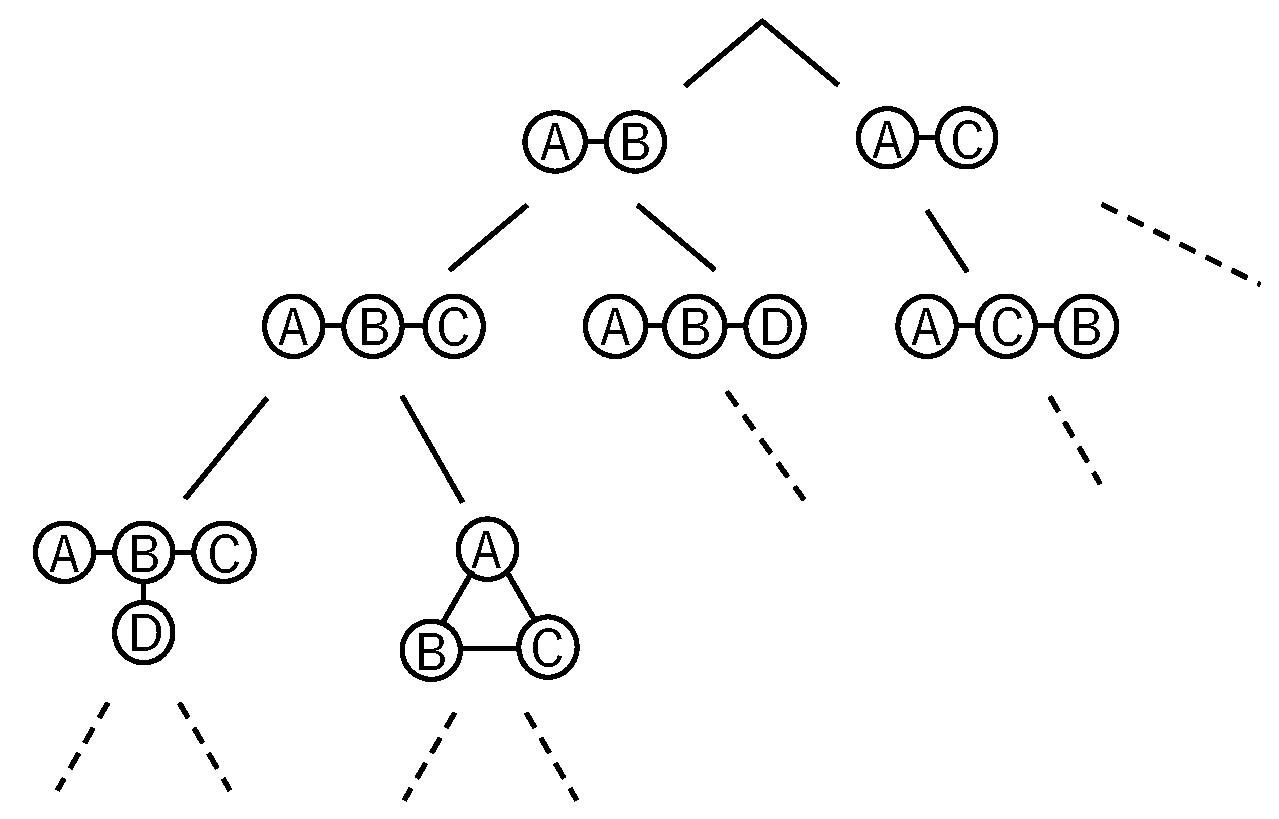
\includegraphics[width=0.5\linewidth]{img/search_tree.eps}
  \caption{DFS code tree. Search space for subgraphs that appear in the training dataset.}
  \label{fig:search_tree}
\end{figure}

The following \textit{anti-monotone} property of
subgraph isomorphism over the DFS code tree on $\S_N$ can be used to
derive the efficient search-space pruning of the gSpan algorithm:
\begin{equation}
  \label{eq:propSubgraph}
  g' \sqsupseteq g, \quad 
  G_i \not \sqsupseteq g \Rightarrow G_i \not\sqsupseteq g'. % period
\end{equation}

\subsection{Discriminative Criterion}
\label{sec:criterion}
In the previous methods, the discriminating power are calculated 
by model-based criterioa or statistical criterioa such as information gain.
In present paper, the discriminating power ($Discriminative Score: DScore$) is defined 
by the following equation.
%\begin{eqnarray}
  %\label{eq:score_C}
  %CScore(g) = \max \Big[ \sum_{n=1}^{N} y_{n} (2\I(G_{n} \sqsupseteq g) - 1), \sum_{n=1}^{N} y_{n} (2\I(G_{n} \not\sqsupseteq g) -1) \Big]
%\end{eqnarray}
%This score is the sum of the values that take +1 if the graph label prediction is correct and -1 otherwise.
%When predicting the graph labels with real values, $RegressionScore$ $(RScore)$ is used defined as (\ref{eq:score_R}).
\begin{eqnarray}
  \label{eq:score_R}
  DScore(g) &=& \tss(\D_1(g)) + \tss(\D_0(g)) \\
  \tss(\D) &=& \sum_{i \in [N]}
  (y_i - \bar{y})^2, \,\, \bar{y} = \frac{1}{N} \sum_{i \in [N]} y_i. \nonumber
\end{eqnarray}
where TSS is the total sum of squared error and
$\D_1(g) = \{ (G_i, y_i) \in \D \mid G \sqsupseteq g \} $ and
$\D_0(g) = \{ (G_i, y_i) \in \D \mid G \not\sqsupseteq g \} $.
Since this score represents an error, 
a larger value indicates lower discriminating power, 
and a smaller value indicates higher discriminating power.
This score does not depend on the learning model, 
and can be used even when the labels are discrete values.


\section{Problem Setting and Challenges}
Our problem is to search for a subgraph $g$
%that maximizes (\ref{eq:score_C}) or minimizes (\ref{eq:score_R}).
that minimizes (\ref{eq:score_R}).
However, the search space of subgraphs (Section \ref{sec:subgraphMining}) is intractably large
due to the combinatorial explosion.
The naive search policy require very high computational costs 
and it is difficult to find the suitable solution.
Our challenge is to design an efficient policy for searching subgraphs in a large search space
based on the discriminative criteria.
%TODO


\section{Depth First Search with Branch and Bound}
State of the art methods \cite{Saigo:2009, Shirakawa:2018} 
searching for a discriminative subgraph pattern is 
based on the depth first search, as shown in Figure \ref{fig:search} (a), with branch and bound.
\cite{Shirakawa:2018} searches the best subgraph pattern using $DScore$. 
This method calculates the bound of child node of search space, 
and if the bound is lower than the provisional solution the child is pruned.
\begin{comment}
\begin{theorem}
  \label{thm:bound_C}
  Given $\D_1(g)$ and $\D_0(g)$, for any subgraph $g' \sqsupseteq g$,
  \begin{multline}
    \label{eq:bound_C}
    CScore(g') \leq 
    \max \Big[ 2 \sum_{\{n | y_n=+1, \{G_{n}, y_{n}\} \in D_1(g)\}} y_n - \sum_{n=1}^{N}y_n, 
	-2 \sum_{\{n | y_n=-1, \{G_{n}, y_{n}\} \in D_1(g)\}} y_n + \sum_{n=1}^{N}y_n \Big]
  \end{multline}
\end{theorem}
\end{comment}

\begin{theorem}
  \label{thm:bound_R}
  Given $\D_1(g)$ and $\D_0(g)$, for any subgraph $g' \sqsupseteq g$,
  \begin{multline}
    \label{eq:bound_R}
    DScore(g') \geq 
    \mymin{(\diamond,k)} \Big[ \tss(\D_1(g) \setminus S_{\diamond, k}) + \tss(\D_0(g) \cup S_{\diamond, k}) \Big]
  \end{multline}
  where $ (\diamond, k) \in \{ \leq, > \} \times \{ 2, \dots, |\D_1(g) - 1| \} $,
  and $S_{\diamond, k} \subset \D_1(g)$, such that $S_{\leq, k}$ is
  a set of $k$ pair $(G_i, r_i)$ selected from $\D_1(g)$ in descending order of residual error $r_i$,
  and $S_{>, k}$ is that in increasing order.
  Note that $\setminus$, $\cup$ are set difference and set union respectively.
\end{theorem}

\begin{proof}
  Given $\D_1(g)$ and $\D_0(g)$,
  \small
  \begin{align}
    \bound &= \mymin{g'} \bigl[ \tss(\D_1(g')) + \tss(\D_0(g'))  \bigr] \notag \\
    \label{eq:boundSubset}
    &= \mymin{S \subset \D_1(g)} \bigl[ \tss(\D_1(g) \setminus S) + \tss(\D_0(g) \cup S)  \bigr] \\
    \label{eq:linearBound}
    &= \mymin{(\diamond,k)} \Big[ \tss(\D_1(g) \setminus S_{\diamond,k}) + \tss(\D_0(g) \cup S_{\diamond,k}) \Big]
  \end{align}\normalsize
  where $ (\diamond, k) \in \{ \leq, > \} \times \{ 2, \dots, |\D_1(g) - 1| \} $.
  From the anti-monotone property \eqref{eq:propSubgraph}, we have
  $\D_1(g') \subseteq \D_1(g)$ for $g' \sqsupseteq g$
  for the training set $\D$ from which the equation \eqref{eq:boundSubset}
  directly follows. Thus, we show \eqref{eq:linearBound} in
  detail. For simplicity,
  let $A =,\{ a_1, \dots, a_n \mid a_i \in \mathbb{R} \}$ denote $\D_1(g)$,
  and $B = \{ b_1, \dots, b_m \mid b_i \in \mathbb{R} \}$ denote $\D_0(g)$.
  Then, the goal of \eqref{eq:boundSubset} is to minimize the total sum
  of squares $\tss(A \setminus S) + \tss(B \cup S)$ by tweaking
  $S = \{ s_1, \dots, s_k \} \subset A$.
  The key fact is that $\tss(A \setminus S) + \tss(B \cup S)$ can
  be regarded as a quadratic equation of $\sum_{i=1}^k s_i$ when the size
  of $S$ is fixed to $k$. More precisely,
  \begingroup
  \allowdisplaybreaks
	\begin{align*}
	  &\tss(A) 
	  = \mysum{n} \Big(a_i - \frac{\mysum{n}a_i}{|A|}\Big)^2
	  = \mysum{n} a_i^2 - \frac{\big(\mysum{n} a_i\big)^2}{|A|} \\
	  &\tss(A) + \tss(B) 
	  = \mysum{n} a_i^2 + \mysum{m} b_i^2 - \frac{\big(\mysum{n} a_i\big)^2}{|A|} - \frac{\big(\mysum{m} b_i\big)^2}{|B|} \\
	  &\tss(A \backslash S) + \tss(B \cup S) \\
	  &= \mysum{n} a_i^2 + \mysum{m} b_i^2 - \frac{\big(\mysum{n} a_i - \mysum{k} s_i\big)^2}{|A \backslash S|} - \frac{\big(\mysum{m} b_i - \mysum{k} s_i\big)^2}{|B \cup S|} \\
	  &= \mysum{n} a_i^2 + \mysum{m} b_i^2 - \frac{\big(\mysum{n} a_i - \mysum{k} s_i\big)^2}{n - k} - \frac{\big(\mysum{m} b_i - \mysum{k} s_i\big)^2}{m + k} \\
	\end{align*}
      \endgroup
      Therefore, $\tss(A \setminus S) + \tss(B \cup S)$ is minimized
      when $\sum_{i=1}^k s_i$ is maximized or minimized. In other words,
      \eqref{eq:boundSubset} becomes minimum when the mean of $S \subset
      \D_1(g)$ is maximized or minimized.
	  \qed
\end{proof}

%TODO
order


\begin{figure}[t]
  	\centering
  	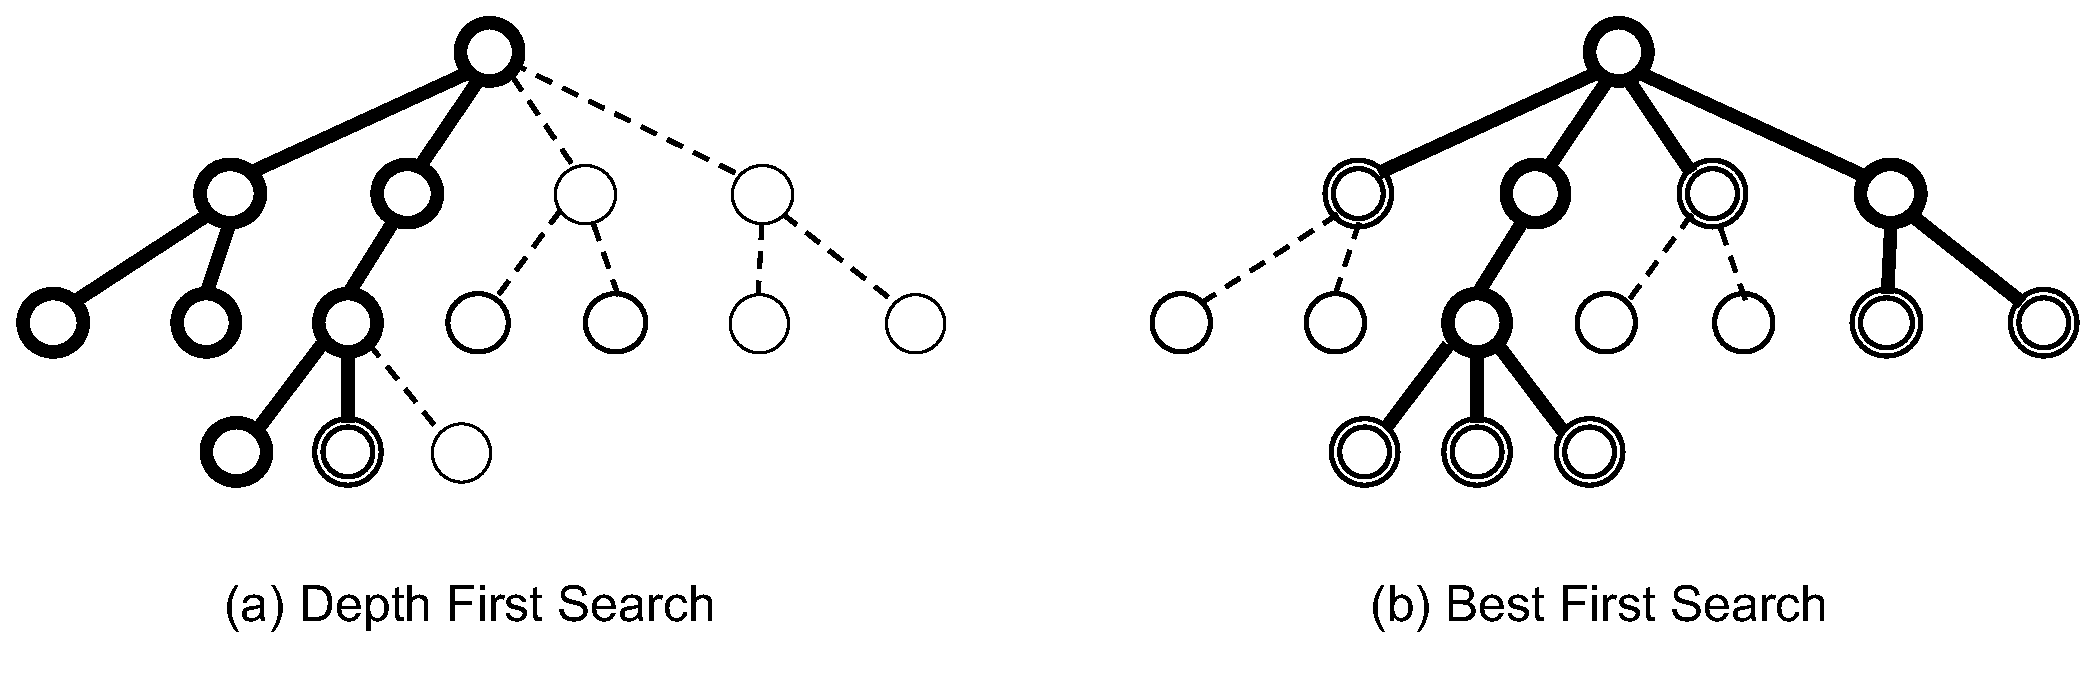
\includegraphics[width=0.9\linewidth]{img/search.eps}
	\caption{
		Depth-first vs. Best-first.
		The bold circles show already searched nodes and 
		double circles show the candidate nodes for next expansion}
  	\label{fig:search}
\end{figure}

\section{Proposed Method}
The previous method \cite{Shirakawa:2018} employs a naive depth-first search policy. 
This policy does not capture factors such as the nature of the dataset or the situation of current search.
The previous method calculate $DScore$ and its lower bound for every subgraph, 
so there is no additional cost for using these values in search policies.
In this section, using these values, 
we propose two efficient search policies 
based on $(i)$ Best-first Search and $(ii)$ Monte Carlo Tree Search.

\subsection{Best-first Search}
Best-first searching \cite{pearl:1984} is a search policy 
that expands from the best node based on some evaluation value, shown as Figure \ref{fig:search} (b).
The A* algorithm \cite{hart:1968} and Dijkstra algorithm \cite{dijkstra:1959} are representative.

The previous method designed the pruning rule 
by calculating the bound value in (\ref{eq:bound_R}). 
In the proposed method, this bound value is set as the search priority of each node, 
and is applied to the best-first search.
The pseudocode is shown in Algorithm.~\ref{alg:bfs}.
The search starts from the root node, 
and selects the node with the highest bound from the expansion candidate set.
The child nodes of the selected node are expanded, 
and the score is calculated and added to the expansion candidate set.
The above operation is repeated until pruning is possible for all expansion candidate set.\\

\begin{algorithm2e}[H]
  \caption{Subgraph Search by Best-first Search}
  \label{alg:bfs}
  \KwIn{Training data $\D = \{ (G_1,r_1), (G_2,r_2), \dots, (G_N,r_N) \} $}
  \KwOut{Best score subgraph $g^*$}
  \Fn{Best-first Search($\D$)}{
	$candidate \leftarrow \{root\}$
    \Repeat{all candidate can be pruned}{
		$g \leftarrow \argmax_{candidate\ c} bound(c)$ \;
		$candidate \leftarrow candidate / {g}$ \;
		\ForAll{child c of g}{
      		\If{DScore(c) is better than $score^*$}{
	  		  $score^*$ $\leftarrow$ $DScore(c)$ \;
	  		  $g^*$ $\leftarrow$ $c$  \;
      		}
			$candidate \leftarrow candidate \cup {c}$ \;
		}
		
    }
    \KwRet{$g^*$} \;
  }
\end{algorithm2e}

\subsection{Monte Carlo Tree Search}
We consider to apply Monte Carlo tree search (MCTS) 
\cite{Levente:2006, Romaric:2010, Cameron:2012} to our problem. 
MCTS is widely known as the method used in computer Go. 
It is also applied in various fields such as feature selection \cite{Romaric:2010}. 
One of them, Upper Confidence Bounds for Tree (UCT) algorithm 
\cite{Levente:2006} is empirically highly evaluated as a way to find good solutions within a limited budget.
This method resolves the exploration-exploitation problem using Upper Confidence Bound (UCB),
which allows to estimate the expected reward of each child.
The simplest UCB policy is called UCB1 and does not require the prior specific knowledge.
The policy selects to search child node $i$ that maximizes
\begin{equation}
  \label{eq:ucb}
  UCB1 = \bar{X}_{i} + C \times \sqrt{\frac{\ln{n}}{2 n_{i}}}
\end{equation}
where $\bar{X}_{i}$ is the average reward from child node $i$, 
$n_{i}$ is the number of times child node $i$ was selected, 
$n$ is the number of times parent node of $i$ was selected,
and $C$ is an exploration constant.
The left term encourages the exploitation of high expected reward child,
and the right term encourages the exploration of less visited child.

The UCT algorithm is an iterative method 
doing the four operations of selection, expansion, 
simulation, and backpropagation up to a predefined computational cost, shown as Figure \ref{fig:MCTS}.
\begin{figure}[t]
  \centering
  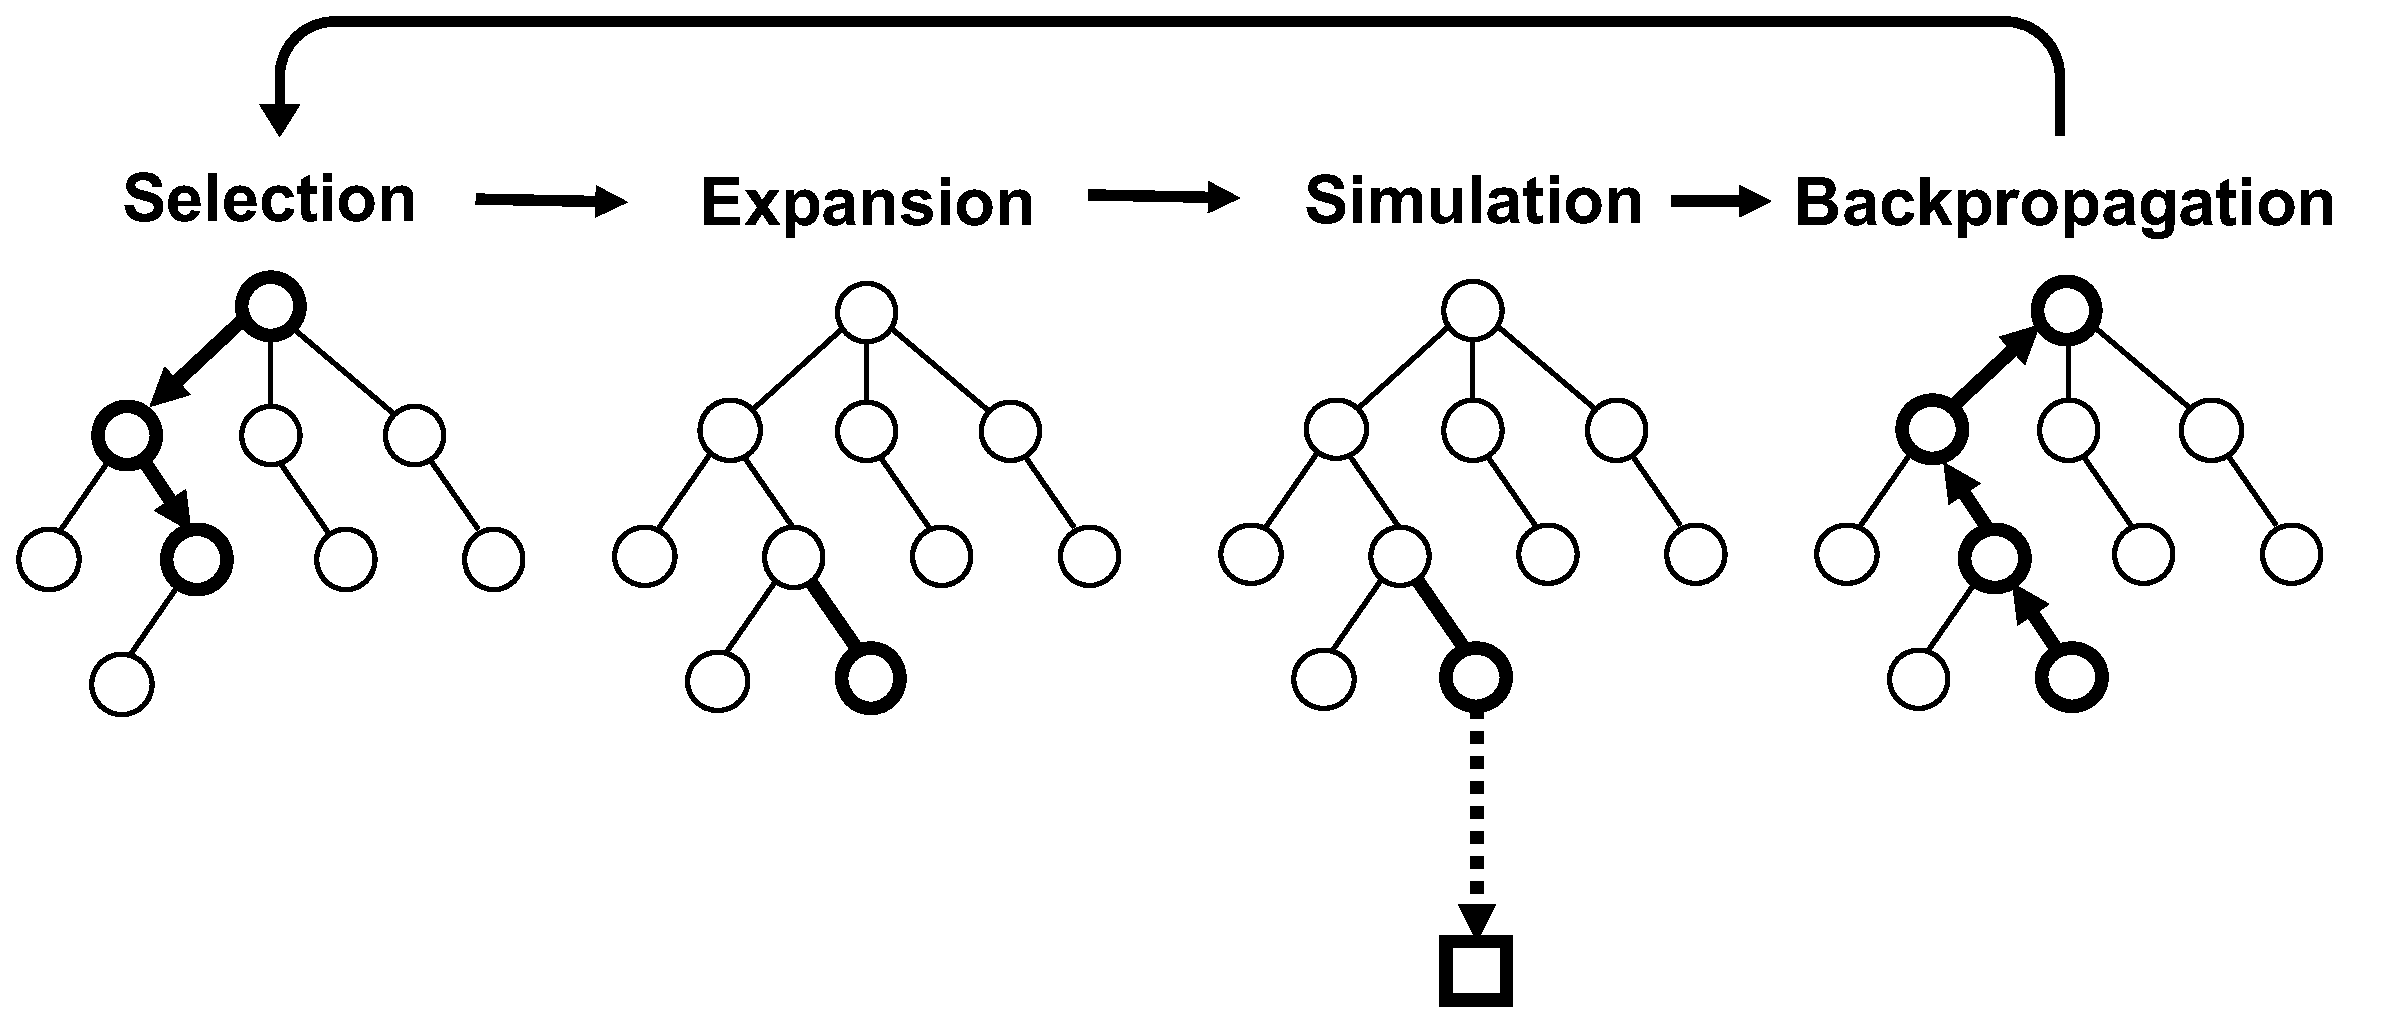
\includegraphics[width=0.9\linewidth]{img/MCTS.eps}
  \caption{One circle of processes in UCT algorithm}
  \label{fig:MCTS}
\end{figure}


\begin{enumerate}
	\item{Selection}:

	~~Start from the root node, and select the child node repeatedly 
	based on the value of $UCB1$ until the expandable node is reached.
	A node is expandable if it represents a non-terminal state and has unvisited children.

	\item{Expansion}:

	~~One random child node that is unvisited is expanded.
	In this operation, we consider the same pruning condition as (\ref{eq:bound_R}). 
	If the random select node can be pruned, another node is reselected and expanded.

	\item{Simulation}:
	
	~~A Monte Carlo simulation is run from the new expanded node,
	and repeatedly select a child randomly from the available children.
	This simulation stops if the simulation node has no children or 
	is based on a stochastic condition known as a stopping feature used in \cite{Romaric:2010}.
	The stochastic condition is $1 - q^{d}$ depending on the simulation node level d,
	where $q < 1$ is a parameter and $q = 1 - 10^{-1}$ in the present paper.
	
	\item{Backpropagation}:

	~~Calculate the reward of the node $g$ obtained by simulation.
	To align the range to $[0, 1]$, reward is defined, 
	\begin{eqnarray}
		reward(g) = -DScore(g) / \tss(\D)
	\end{eqnarray}
	this value will be large if discrimination is successful, otherwise small.
	Then backpropagate this reward to the nodes selected in selection and expansion phase.
\end{enumerate}

%TODO
\subsubsection*{UCT algorithm in Subgraph Feature Space}
UCT algorithm is often used in game-tree space or item set space.
The major difference between these situations 
and the subgraph feature space is the difficulty of constructing the search space.

In this problem setting, the search space is not given in advance.
Therefore, we need to construct a search space that matches the given dataset 
and search for a discriminative subgraph at the same time.

When Monte Carlo simulation is performed in this problem, 
it is necessary to enumerate all the child nodes for each simulation node, which requires a large cost.
We design a low-cost simulation method 
since the simulation cost has a big influence on the search efficiency.

First, a graph including simulation node is randomly selected from the dataset.
Expand the subgraph represented by the simulation node on the selected graph.
If an expanded subgraph is available(minimum order defined by \cite{Yan:2002}), 
this simulation is taken, otherwise it is repeated. \\

The entire procedure of the proposed algorithm is illustrated with pseudocode in 
Algorithm.~\ref{alg:uct}, \ref{alg:four_operations}.\\

\begin{algorithm2e}[H]
  \caption{Subgraph Search by UCT}
  \label{alg:uct}
  \KwIn{Training data $\D = \{ (G_1,r_1), (G_2,r_2), \dots, (G_N,r_N) \} $}
  \KwOut{Best score subgraph $g^*$}
  \Fn{UCT($\D$)}{
    \Repeat{predefined cost is exhausted}{
      \g $\leftarrow $ Selection(root) \;
      \g $\leftarrow $ Expansion(\g) \;
      \If{DScore(g) is better than $score^*$}{
		$score^*$ $\leftarrow$ $DScore(g)$ \;
		$g^*$ $\leftarrow$ \g  \;
      }
      $s \leftarrow $ Simulation(\g) \;
      Backpropagation($s, g$) \;
    }
    \KwRet{$g^*$} \;
  }
\end{algorithm2e}

\begin{algorithm2e}[H]
  \caption{Four Basic Operations in UCT}
  \label{alg:four_operations}
  \Fn{Selection($g$)}{
	\While{$g$ is expandable}{
		$g \leftarrow \argmax_{children\ c\ of\ g} \bar{X}_{c} + C \times \sqrt{\frac{\ln{n_{g}}}{2 n_{c}}}$ \;

	}
    \KwRet{$g$} \;
  }
  \Fn{Expansion($g$)}{
    \Repeat{g' is not pruned}{
	  $g' \leftarrow random(\{children\ c\ of\ g\})$ \;
	}
      \KwRet{$g'$} \;
  }
  \Fn{Simulation($g$)}{
	$s \leftarrow g$ \;
	\While{$s$ has some child and not enough stochastic condition}{
	  \Repeat{$s'$ is enough to minimum order}{
	  	$G \leftarrow random(\D)$ \;
	  	$s' \leftarrow random\ expansion\ from\ s\ on\ G$ \;
	  }
	  $s \leftarrow s'$ \;
	}
      \KwRet{$s$} \;
  }
  \Fn{Backpropagation($s, g$)}{
	$X = reward(s)$ \;
	\While{$g \neq NULL$}{
		$n_{g} \leftarrow n_{g} + 1$ \;
		$\bar{X}_{g} \leftarrow \frac{\bar{X}_{g} \times (n_{g} -1) + X}{n_{g}}$ \;
		$g \leftarrow parent\ of\ g$ \;
	}
  }
\end{algorithm2e}

\section{Experiments}
\subsection{Datasets}
We also evaluate the performance based on the most typical benchmark on real datasets:
the quantitative structure-activity relationship (QSAR). 
We select Four binary-classification datasets (CPDB, Mutag, AIDS(CAvsCM), CAS) in Table~\ref{tbl:dataset}: 
CPDB and Mutag for mutagenicity tests and AIDS(CAvsCM) for antiviral tests.
All chemical structures are encoded as molecular graphs using RDKit\footnote{\url{http://www.rdkit.org/}}, 
and some structures in the raw data are removed by chemical sanitization\footnote{
Due to this pre-processing, the number of datasets differs from that 
in the simple molecular graphs in the literature, 
where the nodes are labeled by atom type, and the edges are labeled by bond type.}.
We simply apply a node labeling by the RDKit default atom invariants (edges not labeled), i.e., 
atom type, \# of non-H neighbors, \# of Hs, charge, isotope, and inRing properties. 
These default atom invariants use connectivity information similar to that used for the well-known 
ECFP family of fingerprints\cite{Rogers:2010}. See \cite{Kearnes2016} for more elaborate encodings.

\tabcolsep = 6pt
\begin{table}[h]
  \centering
  \caption{Real Dataset summary}
  \label{tbl:dataset}
  	\begin{tabular}{lcccc}
		\thickhline
		Dataset			& CPDB           & Mutag        & AIDS(CAvsCM)     & CAS	\\  \hline
		\# data			& 684            & 188          & 1503             & 4337	\\
		\# ($y=-1,+1$)	& (343, 341)     & (63, 125)    & (1081, 422)      & (1936, 2401)	\\  
		\# nodes		& 25.2           & 26.3         & 59.0             & 30.3	\\  
		\# edges		& 25.6           & 28.1         & 61.6             & 31.3	\\  
		\thickhline
		\end{tabular}
  \leftline{\hspace*{2pt} \# of nodes and edges are average.}
\end{table}

In addition to the real datasets, we also have an artificial datasets.
These artificial datasets are made by randomly sampling 100 graphs from CAS, 
which is one of the real data, and assigning a random label to each graph. 
Artificial1 is assigned as a discrete value labels ($y \in \{-1, +1\}$), 
and Artificial2 is assigned as a real value labels ($y \in [-1, +1]$).
Prepare 100 similar datasets for each.
These summary is shown in Table~\ref{tbl:artificial}.
These are used to more generally evaluate each search policy, 
taking into account the settings and properties of various problems.


\tabcolsep = 20pt
\begin{table}[h]
  \centering
  \caption{Artificial Dataset summary}
  \label{tbl:artificial}
  	\begin{tabular}{lcc}
		\thickhline
		Dataset			& Artificial1           & Artificial2        \\  \hline
		\# data			& 100            		& 100          \\
		\# dataset		& 100     	 			& 100    	\\  
		$y$				& $\{-1, +1\}$     	 	& $[-1, +1]$    	\\  
		sampled from			& CAS     	 			& CAS    	\\  
		\thickhline
		\end{tabular}
\end{table}

\subsection{Comparison of Respective Search Efficiency}
First, a feature search is performed once for each artificial dataset without any budget constraint, 
thereby comparing the respective search efficiencies.
Exploration strength parameter of MCTS is set with three type of values (0.1, 1, 10).
Figure~\ref{fig:bestsearch}, \ref{fig:update} are the average results for all 100 datasets, 
which show the number of nodes searched until finding the best subgraph pattern 
and how the provisional solution is updated in each search.
Figure~\ref{fig:bestsearch} shows that MCTS find the best subgraph with the minimum number of searches, 
and the best-first search continues at that point.
In addition, it was found that each search was not significantly affected by the type of graph label, 
and the smaller the value of the MCTS parameter, the better the result.

In Figure~\ref{fig:update}, both of the proposed methods 
can find a good solution faster than the existing depth-first search.
Also the solution is rapidly improved and converged at an early step, 
there is a sufficient expectation for an approximate search under fixed budget constraint.

\begin{figure}[htbp]
 \begin{minipage}{0.5\hsize}
  \begin{center}
   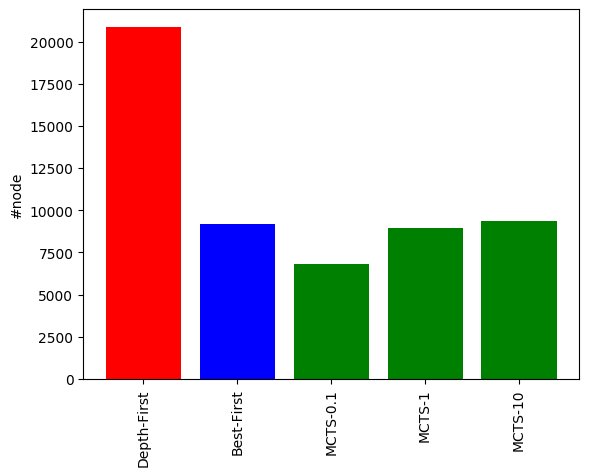
\includegraphics[width=63mm]{img/cas/artificial/1/node.png}
  \end{center}
  \subcaption{Artificial1 ($y \in \{-1, +1\}$)}
 \end{minipage}
 \begin{minipage}{0.5\hsize}
  \begin{center}
   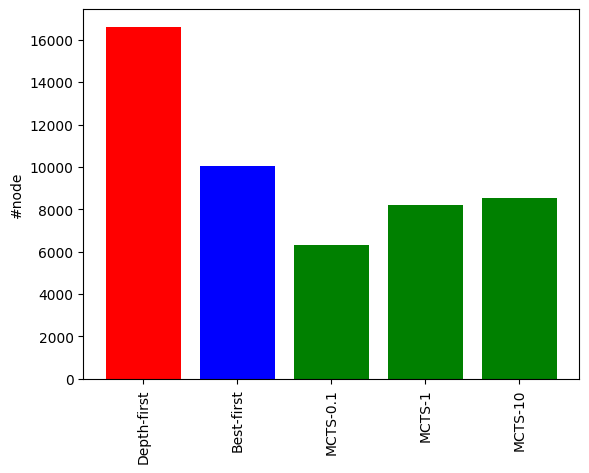
\includegraphics[width=63mm]{img/cas/artificial/2/node.png}
  \end{center}
  \subcaption{Artificial2 ($y \in [-1, +1]$)}
 \end{minipage}
 \caption{Cost comparison until finding the best solution.}
  \label{fig:bestsearch}
\end{figure}

\begin{figure}[htbp]
 \begin{minipage}{0.5\hsize}
  \begin{center}
   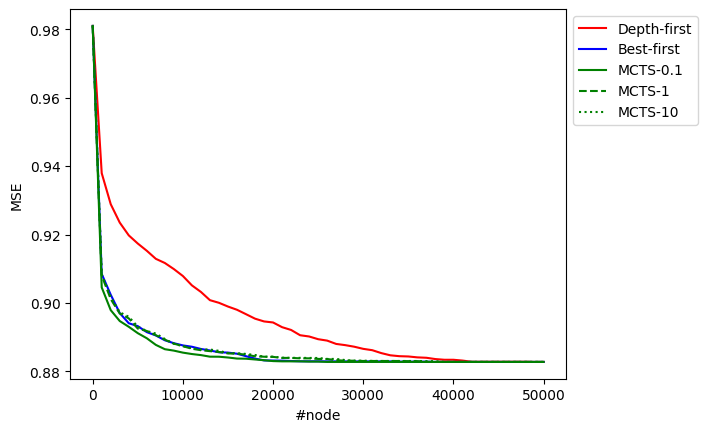
\includegraphics[width=65mm]{img/cas/artificial/1/node_chart.png}
  \end{center}
  \subcaption{Artificial1 ($y \in \{-1, +1\}$)}
 \end{minipage}
 \begin{minipage}{0.5\hsize}
  \begin{center}
   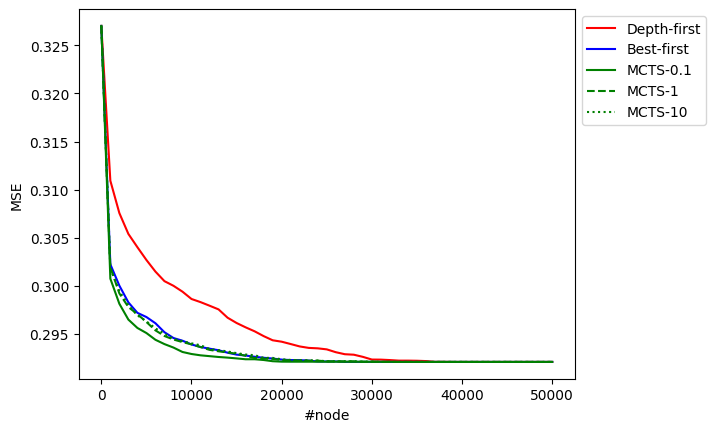
\includegraphics[width=65mm]{img/cas/artificial/2/node_chart.png}
  \end{center}
  \subcaption{Artificial2 ($y \in [-1, +1]$)}
 \end{minipage}
 \caption{Comparison of update of provisional solution.}
  \label{fig:update}
\end{figure}

\subsection{Gradient Tree Boosting with Approximate Search for QSAR}
\label{sec:qsar}
Now that the search efficiency of the proposed method has been confirmed, 
in this part, we construct gradient tree boosting (GTB) \cite{Shirakawa:2018} model for QSAR datasets 
using iterative approximate search of the discriminating subgraphs under fixed budget constraint.
GTB parameters are fixed at the following values,
max subgraph size is 10, the number of trees is 100, depth of each trees is 1 and shrinkage is 1.
The budget constraint on the search is set to 
CPDB=(1000, 2000, 3000, 4000, 5000), Mutag=(200, 400, 600, 800, 1000), 
AIDS(CAvsCM)=(1000, 2000, 3000, 4000, 5000) and CAS=(5000, 10000, 15000, 20000, 25000), 
according to the scale of the dataset, 
and the search is terminated when the number of search nodes exceeds the budget.
The results in Figures~\ref{fig:trainloss} \ref{fig:acc_node} and \ref{fig:acc_time} 
were measured by 10-fold cross validation, 
and Figure~\ref{fig:frequency_time} was measured using all CAS data.

Figure~\ref{fig:trainloss} shows the change in training loss 
of the final ensemble model to the search budget constraint.
Comparing the learning of the model with the same number of searches, 
it can be seen that the model using MCTS performed the best.
For the MCTS exploration strength parameter, 
the same performance is shown, despite the fact that the difference is up to 100 times, 
indicating that the search is robust to this parameter.
The result of the accuracy, is shown in Figure~\ref{fig:acc_node}, 
is similar to the result of the training loss, 
and the accuracy of the model using the MCTS is the highest. 
On the other hand, the approximation search based on the existing depth-first policy 
resulted in poor model accuracy.

Then, we consider the execution time.
Figure~\ref{fig:acc_time} indicates that 
the best-first search requires the longest execution time. 
On the other hand, the execution time of the depth-first search 
is very fast for the same number of searches.
In order to verify this difference in execution time, 
consider the properties of the subgraphs searched by each method.
Figure~\ref{fig:frequency_time} shows the average frequency of the subgraphs searched 
by each method and the execution time.
From Figure~\ref{fig:frequency_time} (a), it can be seen that the subgraphs searched by best-first policy 
have an average frequency 30 times higher than depth-first and 4 times higher than MCTS.
Looking at the lower bound (\ref{eq:bound_R}) in the previous section \ref{sec:previous}, 
the graph with the higher frequency has a larger maximum value of $k$, 
and the lower bound is likely to be larger 
because the movement pattern of many sets can be considered.
In addition, the depth-first policy likely to search for many large subgraphs, 
but the frequency of those is generally low.
Since the calculation of the lower bound requires a linear cost for the frequency, 
there is a large difference in the execution time like Figure~\ref{fig:frequency_time} (b).
The hatched portion of Figure~\ref{fig:frequency_time} (b) indicates the computational cost 
other than the lower bound, and the other portion indicates the computational cost of the bound.
Even if the execution time differs for such a reason, 
the MCTS model showed the best performance 
when the accuracy of the model was evaluated at the same execution time.

\begin{figure}[htbp]
 \begin{minipage}{0.5\hsize}
  \begin{center}
   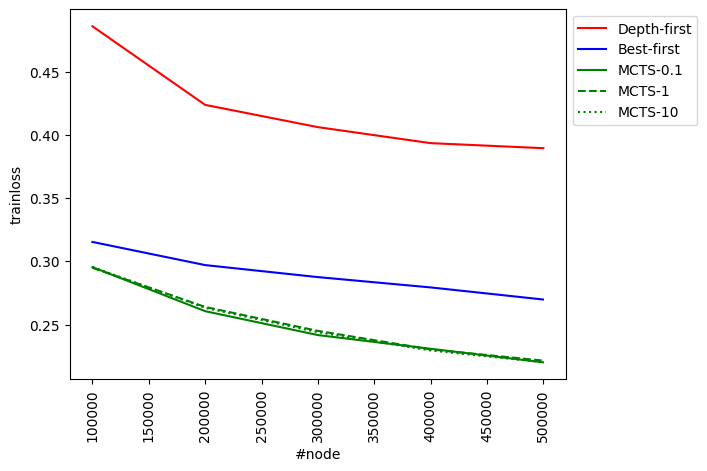
\includegraphics[width=65mm]{img/cpdb/grid/trainloss_node.png}
  \end{center}
  \subcaption{CPDB}
 \end{minipage}
 \begin{minipage}{0.5\hsize}
  \begin{center}
   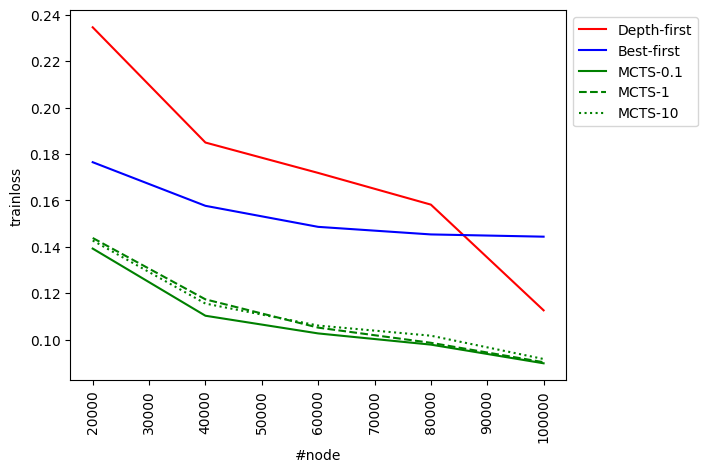
\includegraphics[width=65mm]{img/mutag/grid/trainloss_node.png}
  \end{center}
  \subcaption{Mutag}
 \end{minipage}\\
 \begin{minipage}{0.5\hsize}
  \begin{center}
   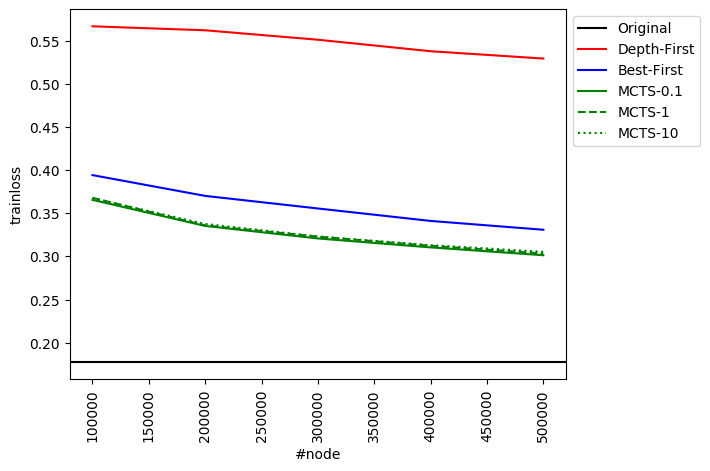
\includegraphics[width=65mm]{img/aids/grid/trainloss_node.png}
  \end{center}
  \subcaption{AIDS}
 \end{minipage}
 \begin{minipage}{0.5\hsize}
  \begin{center}
   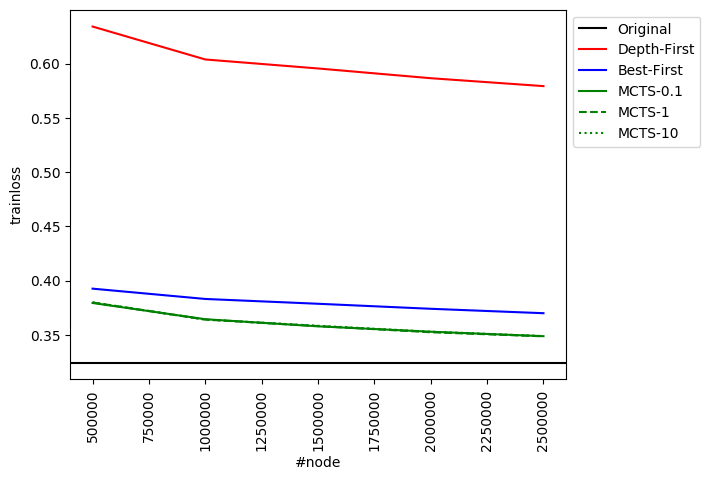
\includegraphics[width=65mm]{img/cas/grid/trainloss_node.png}
  \end{center}
  \subcaption{CAS}
 \end{minipage}
 \caption{Training loss to the number of search nodes for QSAR.}
  \label{fig:trainloss}
\end{figure}

\begin{figure}[htbp]
 \begin{minipage}{0.5\hsize}
  \begin{center}
   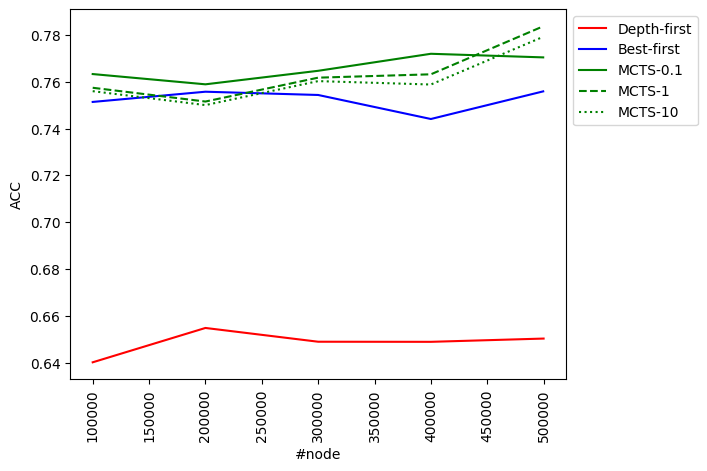
\includegraphics[width=65mm]{img/cpdb/grid/acc_node.png}
  \end{center}
  \subcaption{CPDB}
 \end{minipage}
 \begin{minipage}{0.5\hsize}
  \begin{center}
   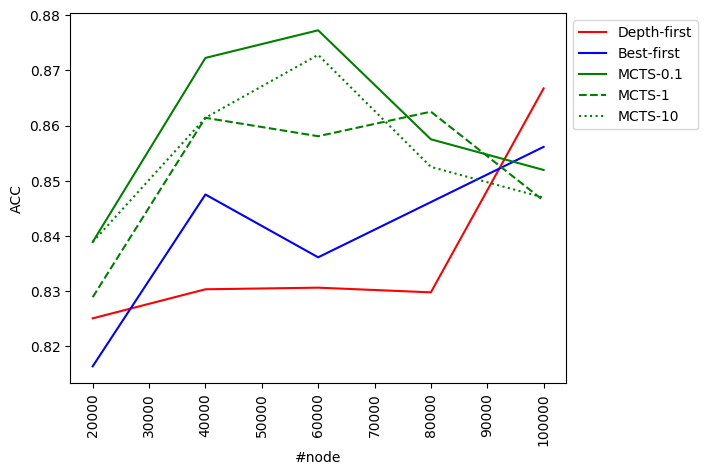
\includegraphics[width=65mm]{img/mutag/grid/acc_node.png}
  \end{center}
  \subcaption{Mutag}
 \end{minipage}\\
 \begin{minipage}{0.5\hsize}
  \begin{center}
   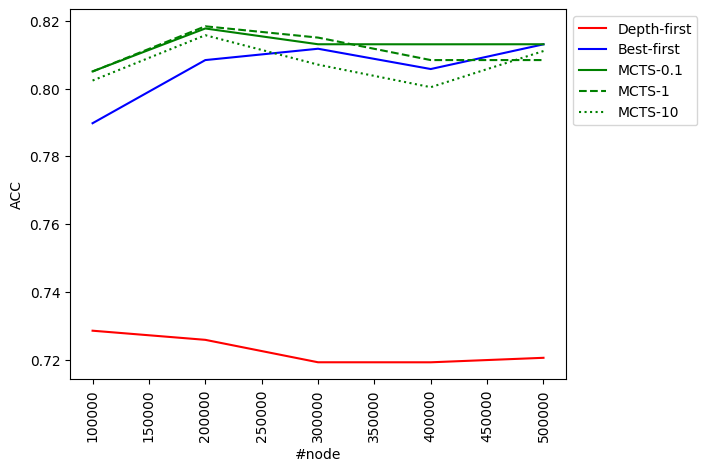
\includegraphics[width=65mm]{img/aids/grid/acc_node.png}
  \end{center}
  \subcaption{AIDS}
 \end{minipage}
 \begin{minipage}{0.5\hsize}
  \begin{center}
   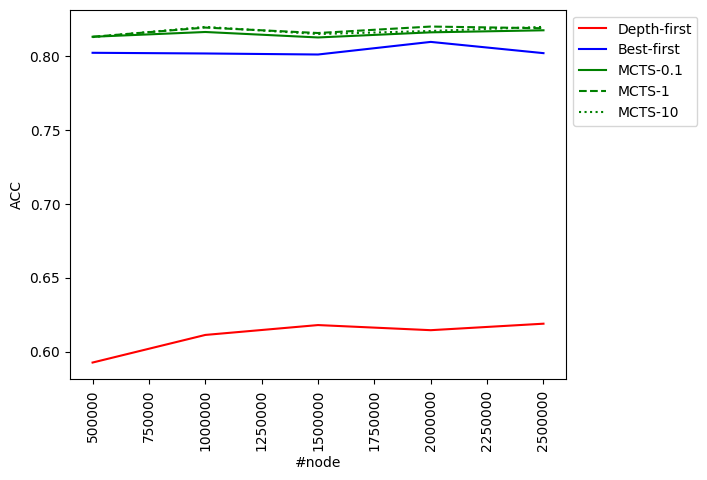
\includegraphics[width=65mm]{img/cas/grid/acc_node.png}
  \end{center}
  \subcaption{CAS}
 \end{minipage}
 \caption{Test accuracy to the number of search nodes for QSAR.}
  \label{fig:acc_node}
\end{figure}

\begin{figure}[htbp]
 \begin{minipage}{0.5\hsize}
  \begin{center}
   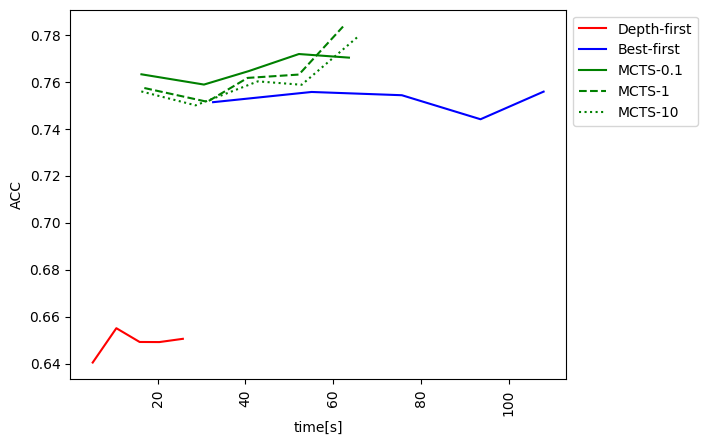
\includegraphics[width=65mm]{img/cpdb/grid/acc_time.png}
  \end{center}
  \subcaption{CPDB}
 \end{minipage}
 \begin{minipage}{0.5\hsize}
  \begin{center}
   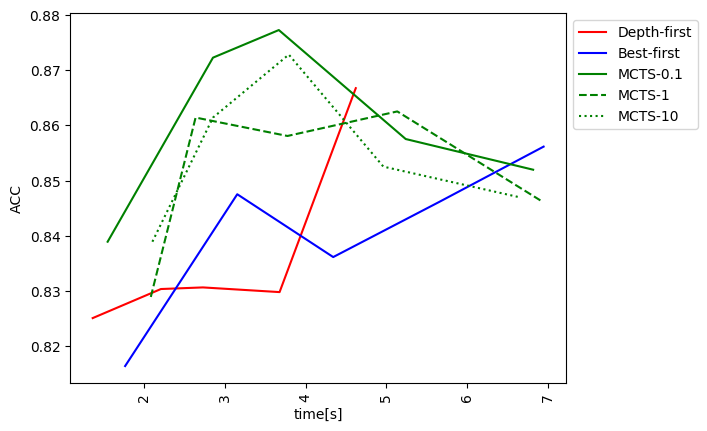
\includegraphics[width=65mm]{img/mutag/grid/acc_time.png}
  \end{center}
  \subcaption{Mutag}
 \end{minipage}\\
 \begin{minipage}{0.5\hsize}
  \begin{center}
   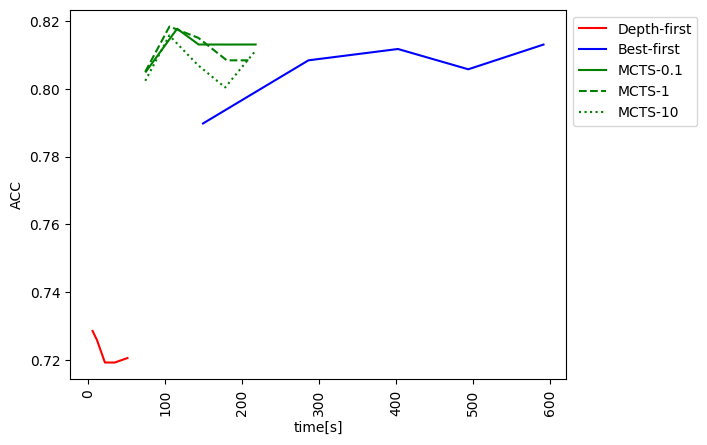
\includegraphics[width=65mm]{img/aids/grid/acc_time.png}
  \end{center}
  \subcaption{AIDS}
 \end{minipage}
 \begin{minipage}{0.5\hsize}
  \begin{center}
   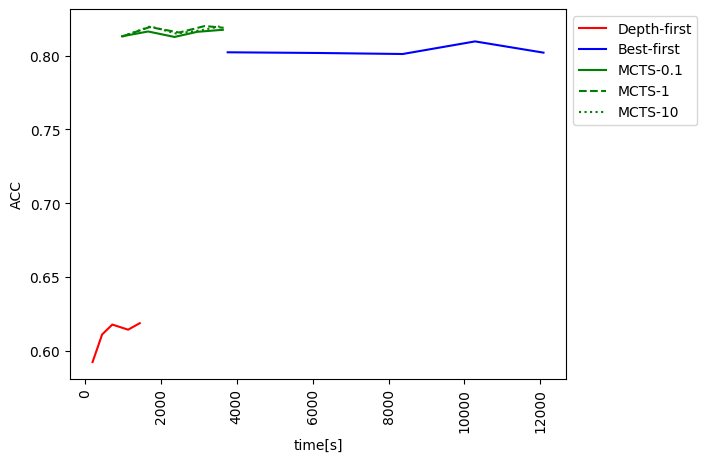
\includegraphics[width=65mm]{img/cas/grid/acc_time.png}
  \end{center}
  \subcaption{CAS}
 \end{minipage}
 \caption{Test accuracy to execution time for QSAR.}
  \label{fig:acc_time}
\end{figure}

\begin{figure}[htbp]
 \begin{minipage}{0.5\hsize}
  \begin{center}
   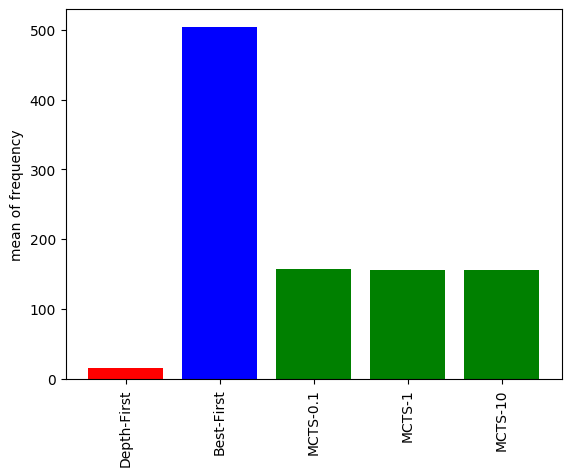
\includegraphics[width=65mm]{img/frequency.png}
  \subcaption{Average frequency of searched subgraphs.}
  \end{center}
  \label{fig:frequency}
 \end{minipage}
 \begin{minipage}{0.5\hsize}
  \begin{center}
   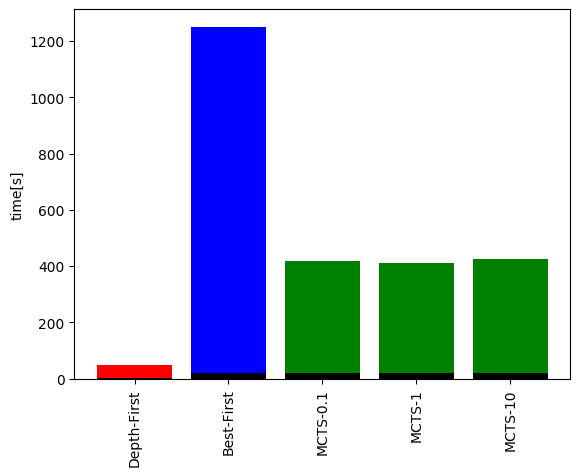
\includegraphics[width=65mm]{img/time.png}
  \subcaption{Execution time of each search.\\ }
  \end{center}
  \label{fig:time}
 \end{minipage}
 \caption{Relationship between execution time and frequency of searched subgraphs for CAS.}
  \label{fig:frequency_time}
\end{figure}

\subsection{Approximate Search vs. Exact Search for Learning}
So far, we have considered the efficiency of each approximate search.
Then, we compare the approximate search with the exact search.
Since approximate search based on MCTS policy performed the best 
compared with other approximate search methods, 
this section compares GTB+MCTS with the existing method \cite{Shirakawa:2018}, GTB+exact Depth-first
The same parameters of GTB and budget constraint are used as for \ref{sec:qsar}
and compared using the test accuracy of 10-fold cross-validation for QSAR datasets.
The results are shown in Table~\ref{tbl:acc} 
and the best MCTS parameters used in the results are shown in Table~\ref{tbl:bestParam}.
Table~\ref{tbl:acc} shows that, the accuracy of GTB+MCTS was $0.4\%~2.7\%$ higher than 
the accuracy of GTB+exact Depth-first.
In addition, the number of search nodes and execution time were reduced from about $1/10$ to $1/200$.
Why did the accuracy of learning improve despite under budget constrain?
Figure~\ref{fig:feature_rate} shows the answer.
This figure indicates the percentage of subgraph size used for learning,
and it can be seen that model based on the exact Depth-first is learned with almost large features.
In particular, 40\% or more of the maximum size feature is used.
This is apparently over-fitting and led to a decrease in accuracy.
On the other hand, model based on MCTS (approximate search) is built with a good balance of features.
The latter is considered to be a better model in terms of generalization performance.

\tabcolsep = 10pt
\begin{table*}[t]
  \centering
  \caption{exact Depth-first vs. MCTS (approximate search).}
  \label{tbl:acc}
  \scalebox{0.90}{
  	 \begin{tabular}{lccc}
  	   \thickhline
  	   Dataset		& ~								& \# Search nodes					& ~			\\
  	   ~   			& GTB+exact Depth-first			& GTB+MCTS       			& Ratio \\ \hline
  	   CPDB 		& $7.2 \times 10^6$				& $5.0 \times 10^5$ 				&  $0.070$  \\
  	   Mutag 		& $3.8 \times 10^5$				& $6.0 \times 10^4$ 				&  $0.015$  \\
  	   AIDS(CAvsCM)	& $7.9 \times 10^7$				& $2.0 \times 10^5$ 				&  $0.003$  \\
  	   CAS	 		& $6.9 \times 10^7$				& $2.0 \times 10^6$ 				&  $0.029$  \\
  	   \thickhline
  	  		 		& ~								& Execution time [s]				& ~			\\
  	   ~   			& GTB+exact Depth-first			& GTB+MCTS       			& Ratio \\ \hline
  	   CPDB 		& $8.2 \times 10^2$				& $6.2 \times 10$	 				&  $0.076$  \\
  	   Mutag 		& $2.3 \times 10^2$				& $3.7$				 				&  $0.016$  \\
  	   AIDS(CAvsCM)	& $2.5 \times 10^4$				& $1.1 \times 10^2$ 				&  $0.004$  \\
  	   CAS	 		& $8.0 \times 10^4$				& $1.7 \times 10^3$ 				&  $0.040$  \\
  	   \thickhline
  	   				& ~								& Accuracy [\%]						& ~			\\
  	   ~   			& GTB+exact Depth-first			& GTB+MCTS       			& Difference \\ \hline
  	   CPDB 		& $77.78$						& $78.35$			 				&  $+0.57$  \\
  	   Mutag 		& $85.03$						& $87.73$			 				&  $+2.70$  \\
  	   AIDS(CAvsCM)	& $81.37$						& $81.84$ 							&  $+0.47$  \\
  	   CAS	 		& $80.82$						& $81.99$		 					&  $+1.17$  \\
  	   \thickhline
  	 \end{tabular}
  }
\end{table*}

\tabcolsep = 14pt
\begin{table*}[t]
  \centering
  \caption{Best budget constraint and exploration strength parameter.}
  \label{tbl:bestParam}
  	\scalebox{0.90}{
  	\begin{tabular}{lcccc}
  	  \thickhline
  	  ~                    	& CPDB     	& Mutag 	& AID(CAvsCM) 	& CAS  		\\  \hline
  	  budget constraint    	& $5000$ 	& $600$ 	& $2000$  		& $20000$		\\  
  	  exploration strength  & $1$ 		& $0.1$		& $1$ 	 		& $1$			\\ 
  	  \thickhline
  	\end{tabular}
  }
\end{table*}

\begin{figure}[htbp]
  \begin{center}
   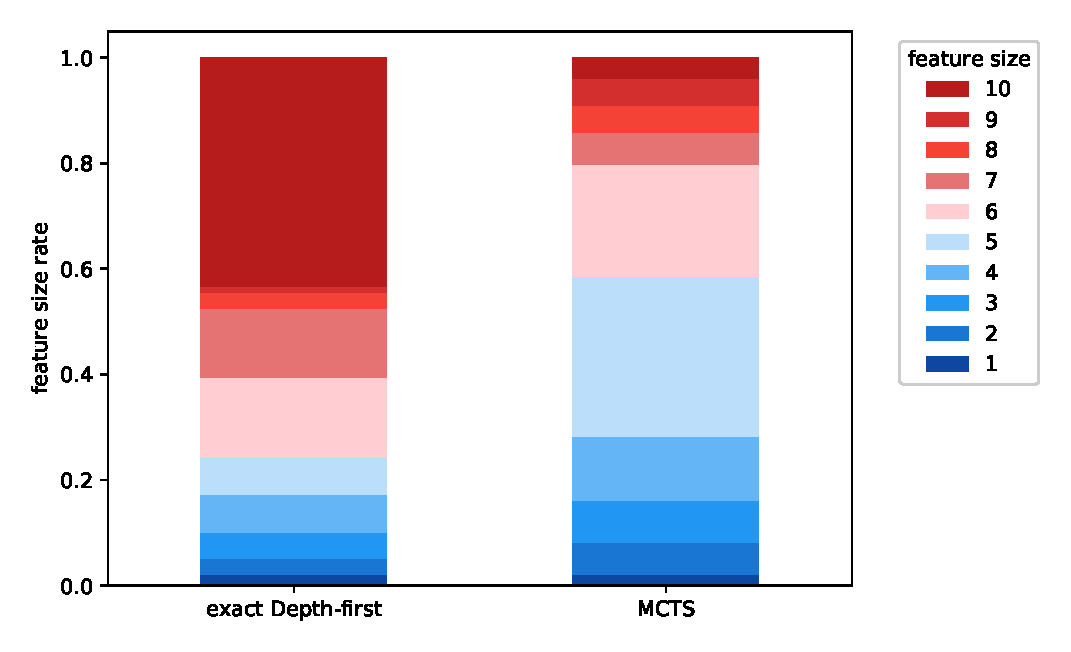
\includegraphics[width=95mm]{img/feature_rate.eps}
  \end{center}
 \caption{The size ratio of the features used for learning the MCTS (approximate search) and the exact Depth-first search.}
  \label{fig:feature_rate}
\end{figure}


\section{Conclusion}
In summary, we proposed an efficient approximate search method 
by applying the MCTS algorithm and the best-first search algorithm to the subgraph feature space.
These approximate search methods were able to obtain better solutions compared 
to existing naive search policy.
In addition, the learning model constructed by performing this search iteratively 
reduced the model construction cost from about 1/10 to 1/200 
while improving the accuracy compared to the existing exact search model.
This confirms that the approximate search leads to an improvement in the generalization performance, 
and may not only reduce the search cost but also provide a good solution for regularization.

However there are many challenges.
First, regarding cost constraint, 
there is no standard as to how much cost should be spent on a problem of what scale.
Currently, it is only experimentally determined, 
so it is easier to handle if the standard is set theoretically.
Second, the MCTS method used this paper is the most basic one. 
Considering more advanced methods and problem-specific heuristics will likely lead to better searches.

\begin{comment}
In summary, we proposed a novel efficient algorithm to learn the nonlinear model 
using subgraph indicators without any class constraint.
In addition to solving computational cost problems, 
our algorithm using MCTS improves generalization ability compared to previous methods.
The search efficiency and prediction accuracy were empirically evaluated by experiments using real datasets.

On the other hand, it is still necessary to investigate the proposed method. 
In this paper, we set the number of Monte Carlo simulations empirically, and there is no uniform standard.
Some MCTS methods may provide theoretical guarantees for searching.
Furthermore, the performance may be improved by adopting some advanced methods of MCTS 
and domain specific heuristics.
\end{comment}


\newpage
\section*{acknowlege}

 
\newpage
\small
%\bibliographystyle{prml}
\bibliographystyle{junsrt}
\bibliography{ref}

\small
\appendix
\input{appendix}

\end{document}
